\section{Introduction to radio interferometric imaging}\label{radio}
%This Section gives an introduction to radio interferometric imaging. We introduce how the interferometer measures visibilities, what problems arise and how reconstruction algorithms solve them. 

A radio interferometer consists of several antennas. Each antenna pair measures a visibility in Fourier space. Each measurement consists of an amplitude and phase at a location at a $u$ and $v$  location. The distance between the antennas, which we call the baseline, defines what point in the Fourier space gets sampled. The Figure \ref{radio:sampling:ants} shows the antenna layout of the MeerKAT radio interferometer, and the Figure \ref{radio:sampling:pattern} shows the measurement points in Fourier space. Short baselines sample points close to the origin, and contain the low-frequency Fourier components. They contain information about large areas of the images. Longer baselines measure points further away from the origin. They sample the high-frequency Fourier components. They contain information about edges, and other small structures in the image.


\begin{figure}[!h]
	\centering
	\begin{subfigure}[b]{0.4\linewidth}
		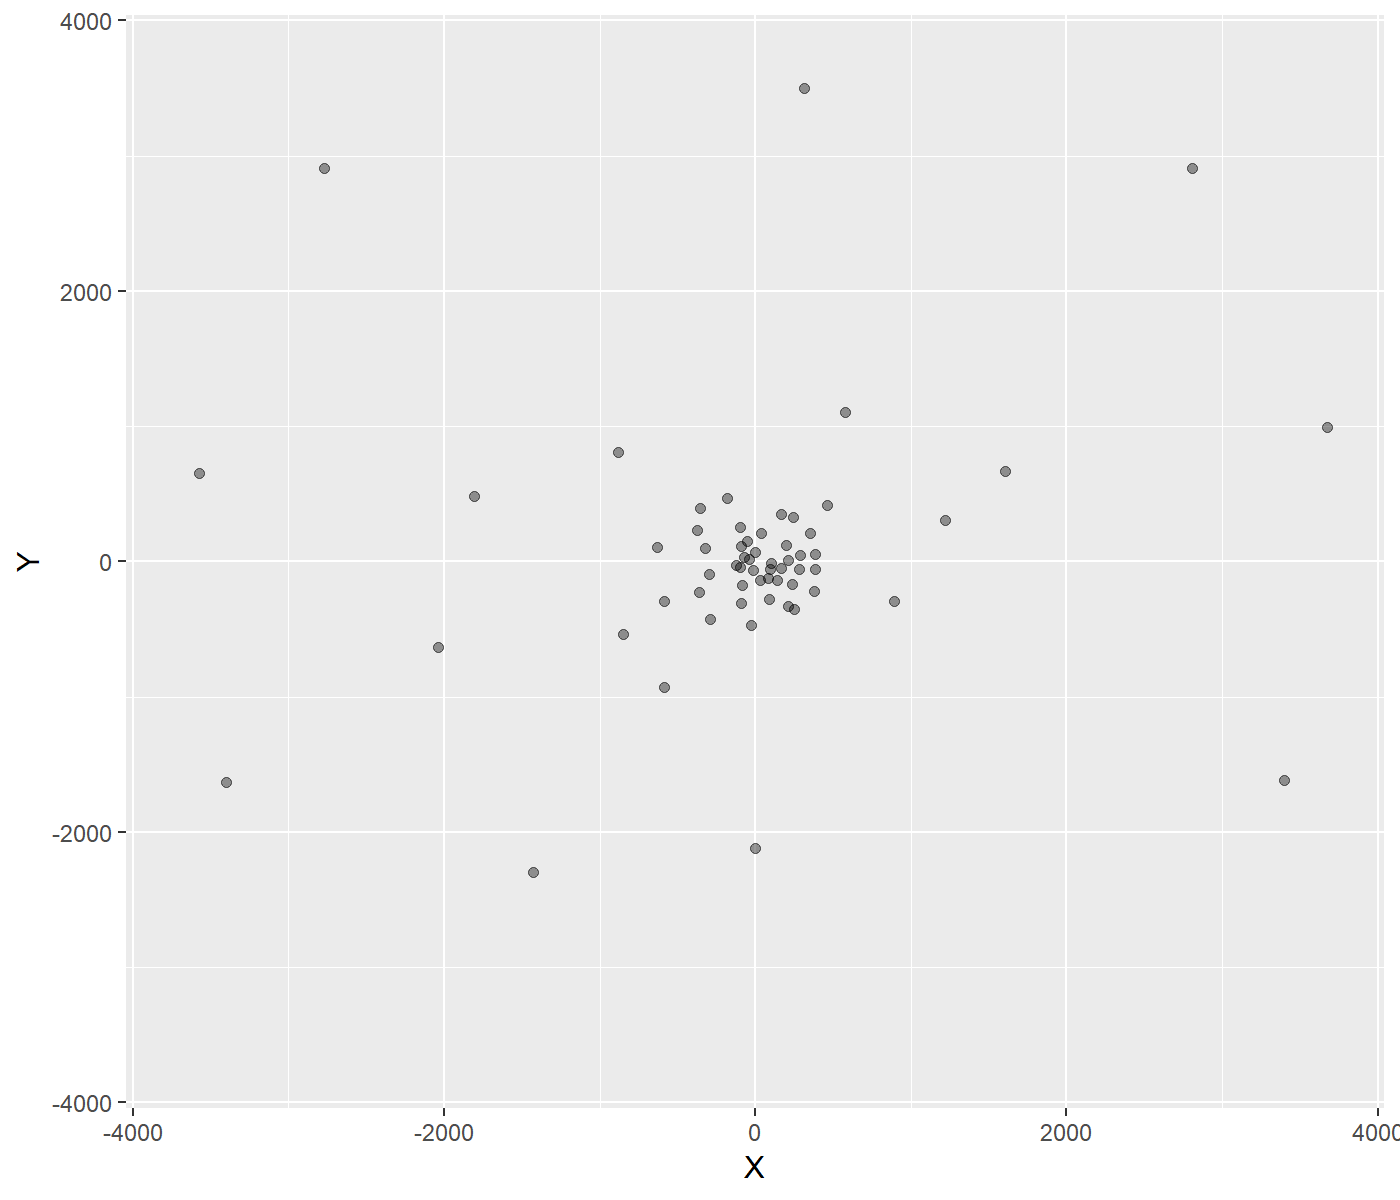
\includegraphics[width=\linewidth]{./chapters/01.intro/aperture/ants.png}
		\caption{Antenna layout.}
		\label{radio:sampling:ants}
	\end{subfigure}
	\begin{subfigure}[b]{0.4\linewidth}
		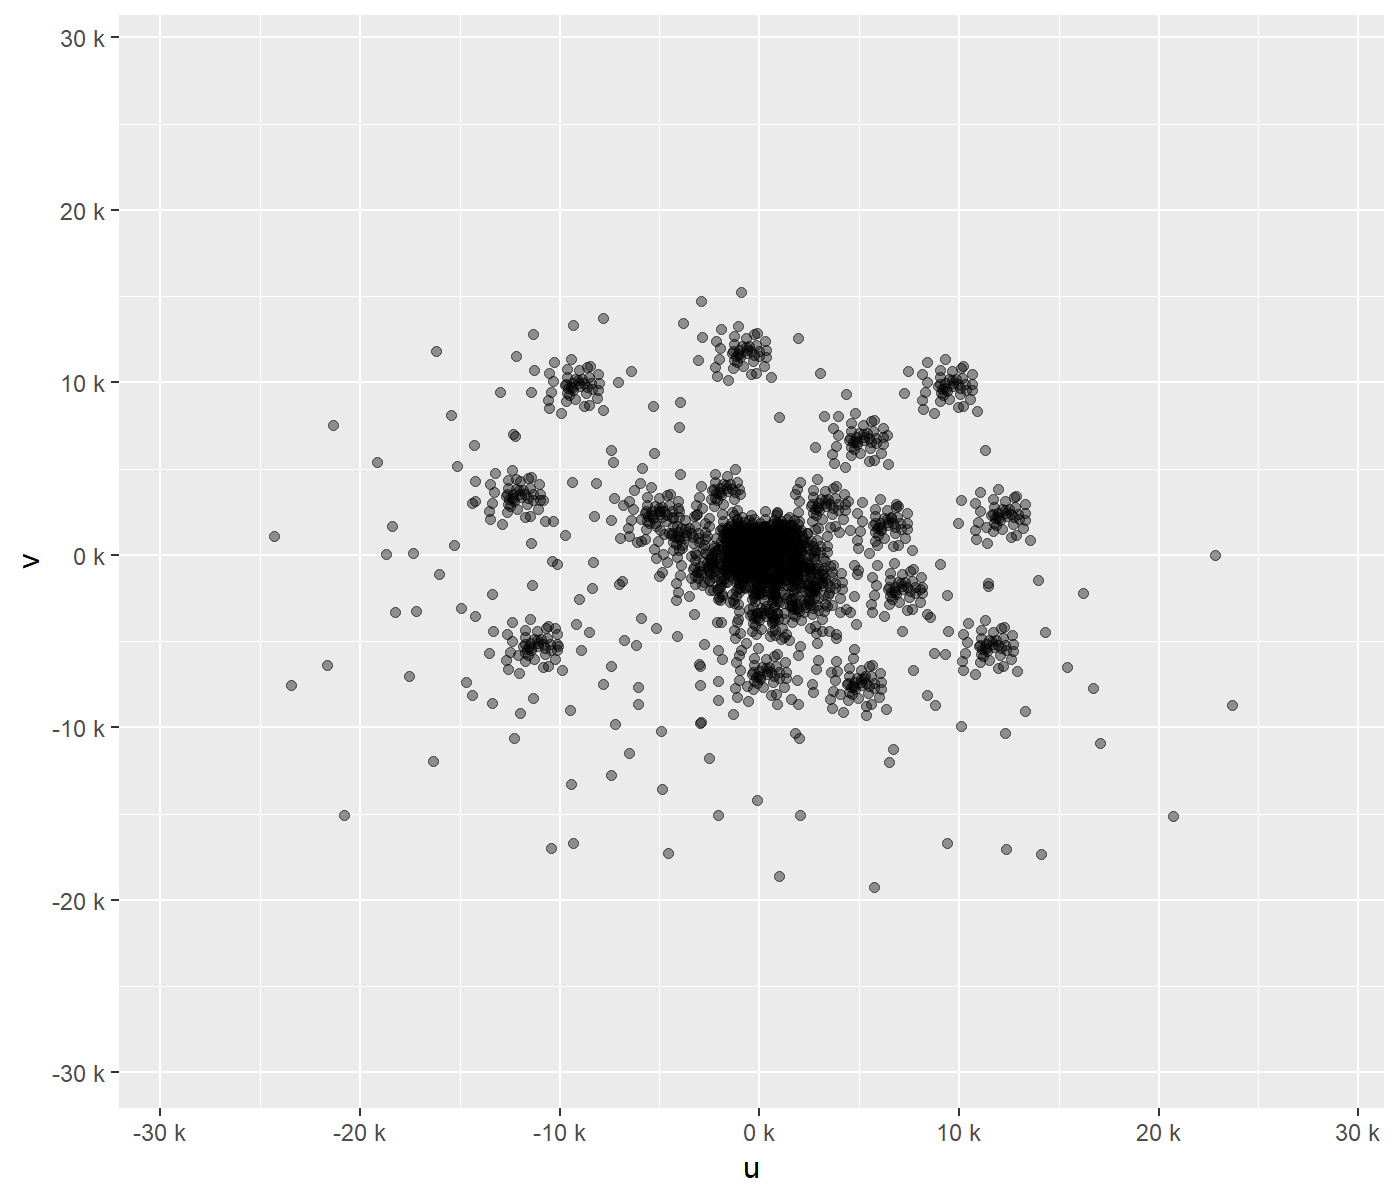
\includegraphics[width=\linewidth]{./chapters/01.intro/aperture/snapshot.png}
		\caption{Visibility sampling pattern.}
		\label{radio:sampling:pattern}
	\end{subfigure}
	\\
	\begin{subfigure}[b]{0.47\linewidth}
		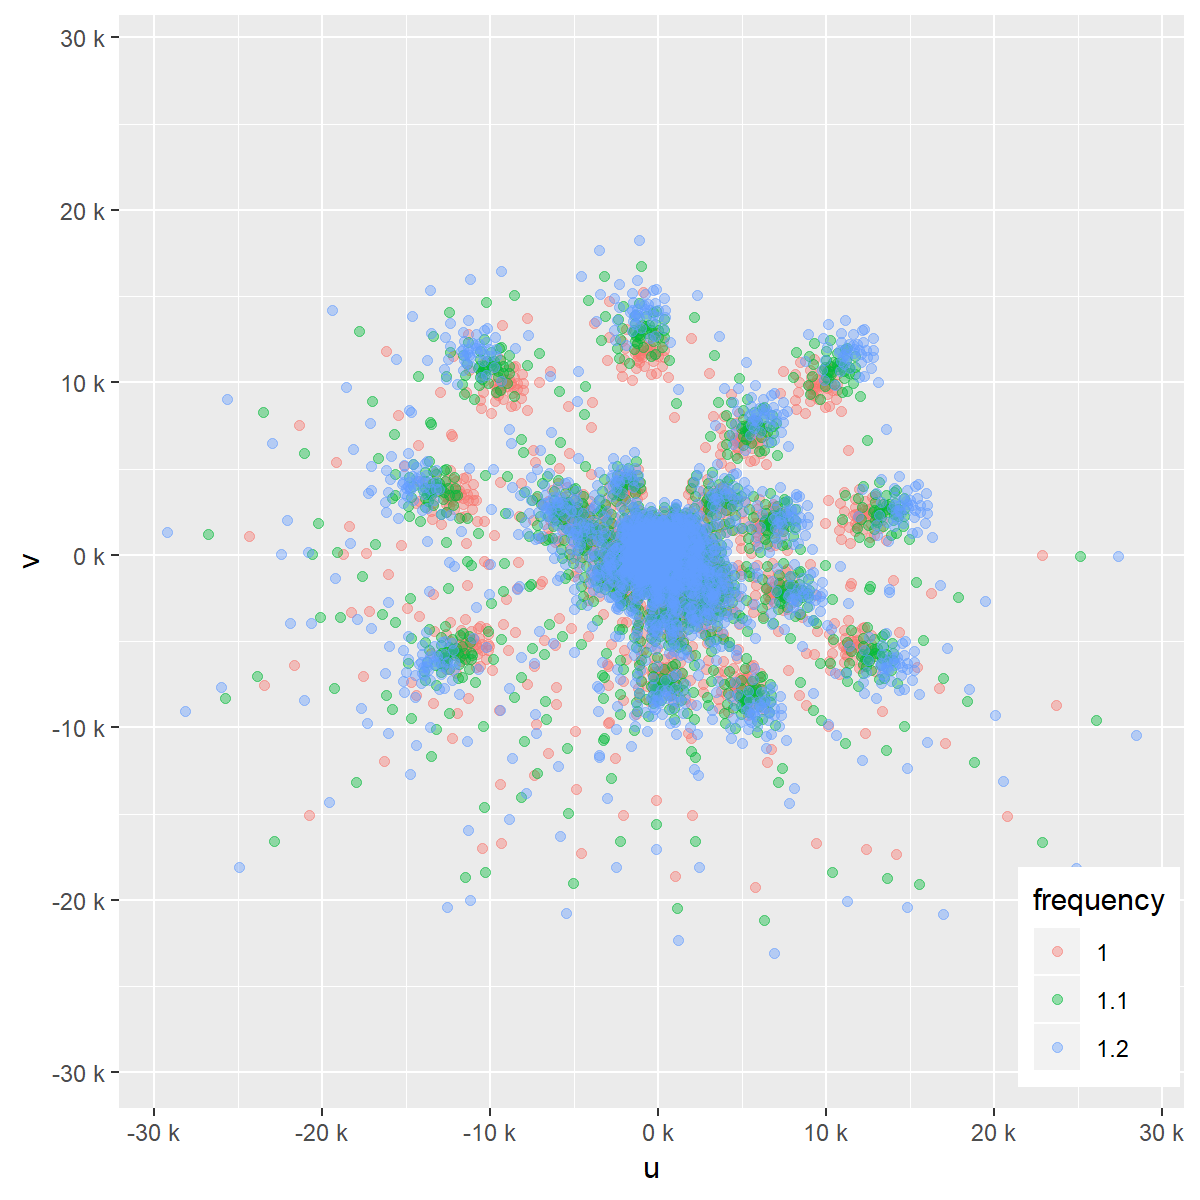
\includegraphics[width=\linewidth]{./chapters/01.intro/aperture/frequencies.png}
		\caption{Visibilities added from multiple channels.}
		\label{radio:sampling:freq}
	\end{subfigure}
	\begin{subfigure}[b]{0.47\linewidth}
		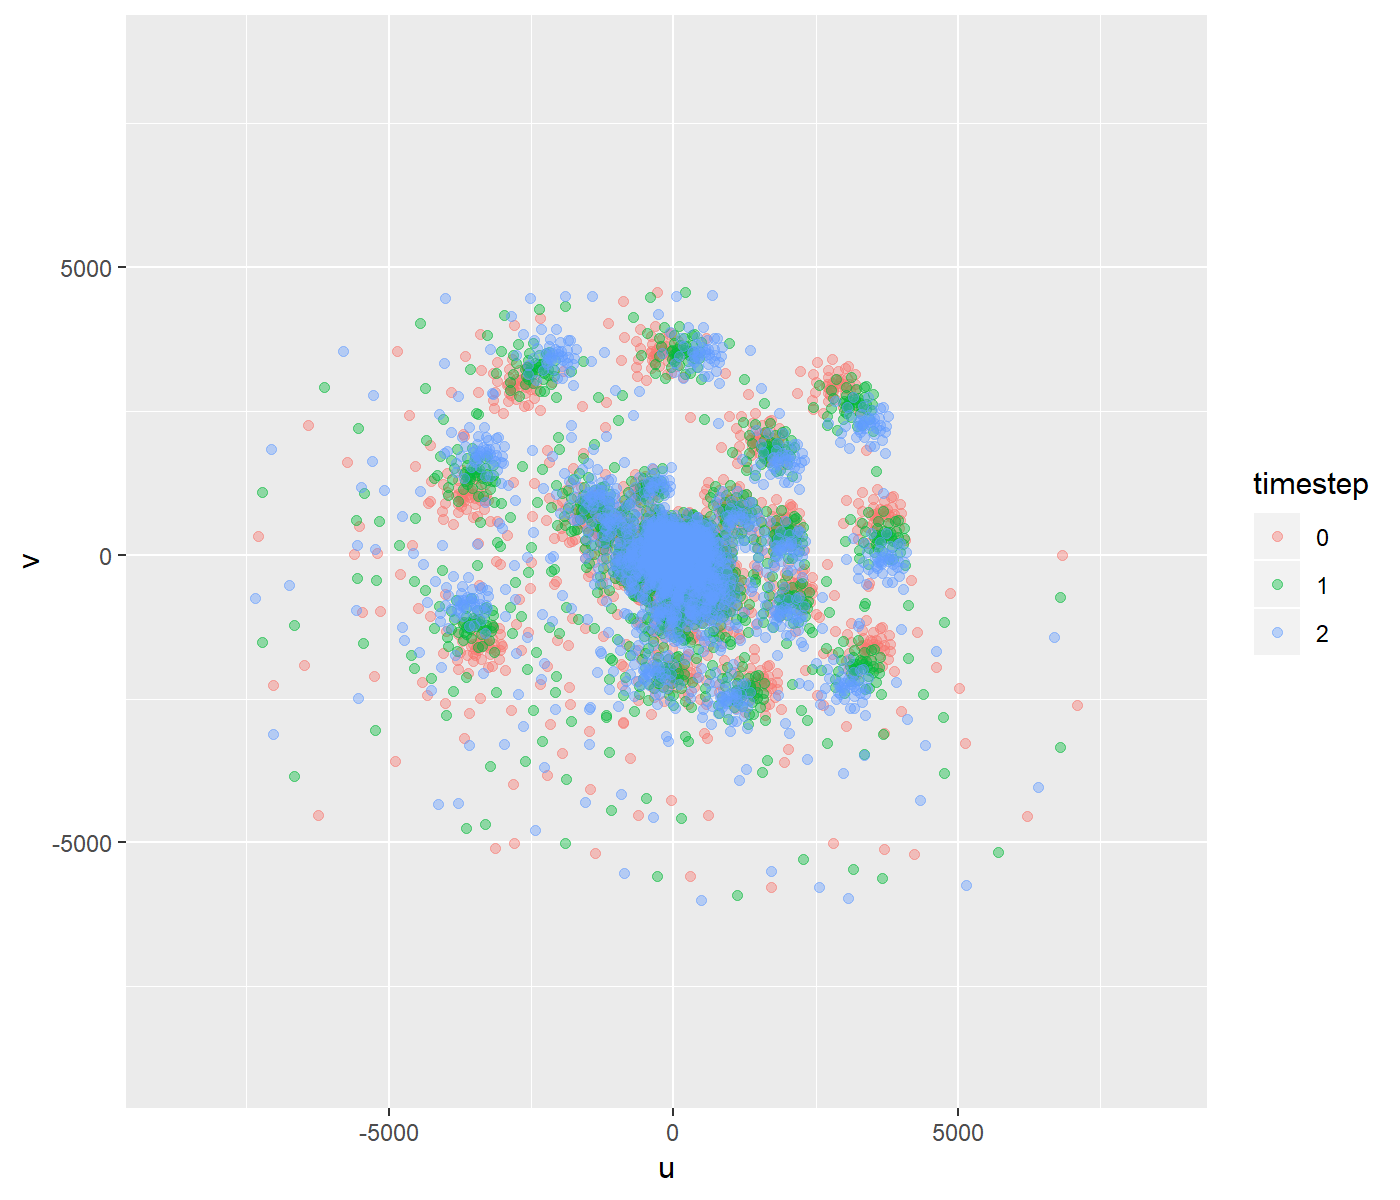
\includegraphics[width=\linewidth]{./chapters/01.intro/aperture/timesteps.png}
		\caption{Visibilities added from multiple timesteps.}
		\label{radio:sampling:time}
	\end{subfigure}
	
	\caption{Sampling regime of the MeerKAT radio interferometer.}
	\label{intro:sampling}
\end{figure}

The sampling pattern of the MeerKAT interferometer is not uniform in the Fourier space. We have areas which are densely sampled, and areas which are sparsely sampled. Note that we only have a few samples of the high-frequency Fourier components. We are missing measurements from a large portion of the Fourier space.

Radio interferometers use two "tricks" to measure more points in the Fourier space. Radio interferometers measure the sky in different radio channels simultaneously. We can add the visibility measurements from different channels together, shown in Figure \ref{radio:sampling:freq}. Each channel measures the Fourier space using the same pattern, but scaled by the radio frequency. 

The second trick is to use the earth's rotation to sample different points in the Fourier space. The earth's rotation also rotates the sampling pattern in Fourier space, shown in Figure \ref{radio:sampling:time}, and we can sample the Fourier space at new locations.

The MeerKAT radio interferometer measures 2016 visibilities, for each channel, at each timestep. It has 20 thousand radio channels. The time resolution can be as low as half a second. This results in roughly 80 million visibility measurements per second. In radio astronomy, we want to reconstruct several hours worth of visibility measurements. 
%GB and TB of data

\begin{figure}[htp]
	% preliminary
	\sbox\twosubbox{%
		\resizebox{\dimexpr.9\textwidth-1em}{!}{%
			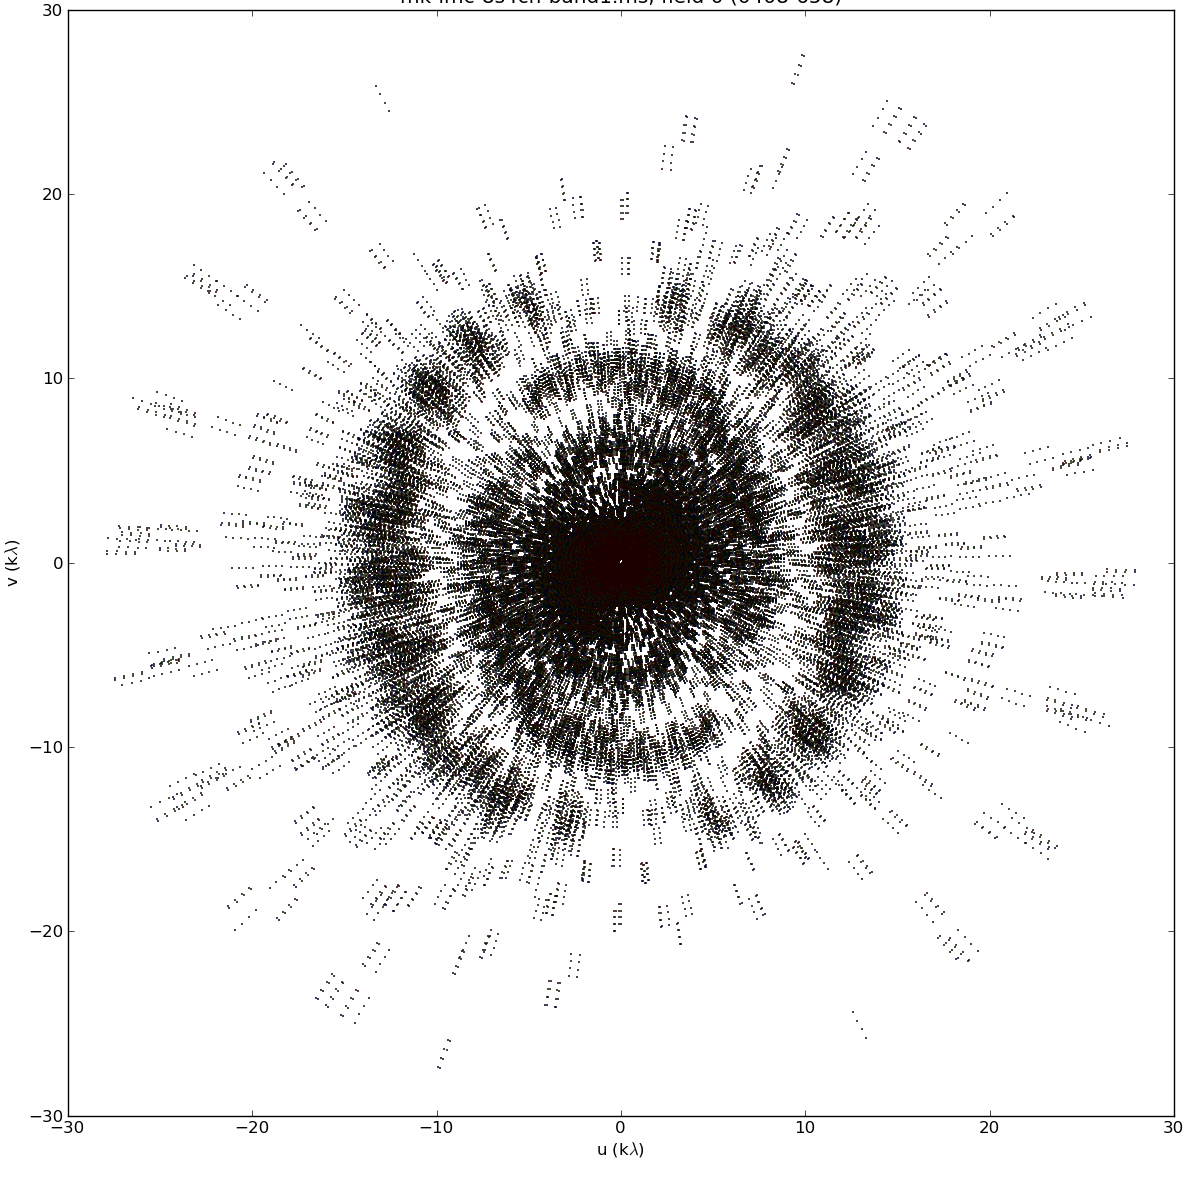
\includegraphics[height=3cm]{./chapters/01.intro/meerkat_uv2.png}%
			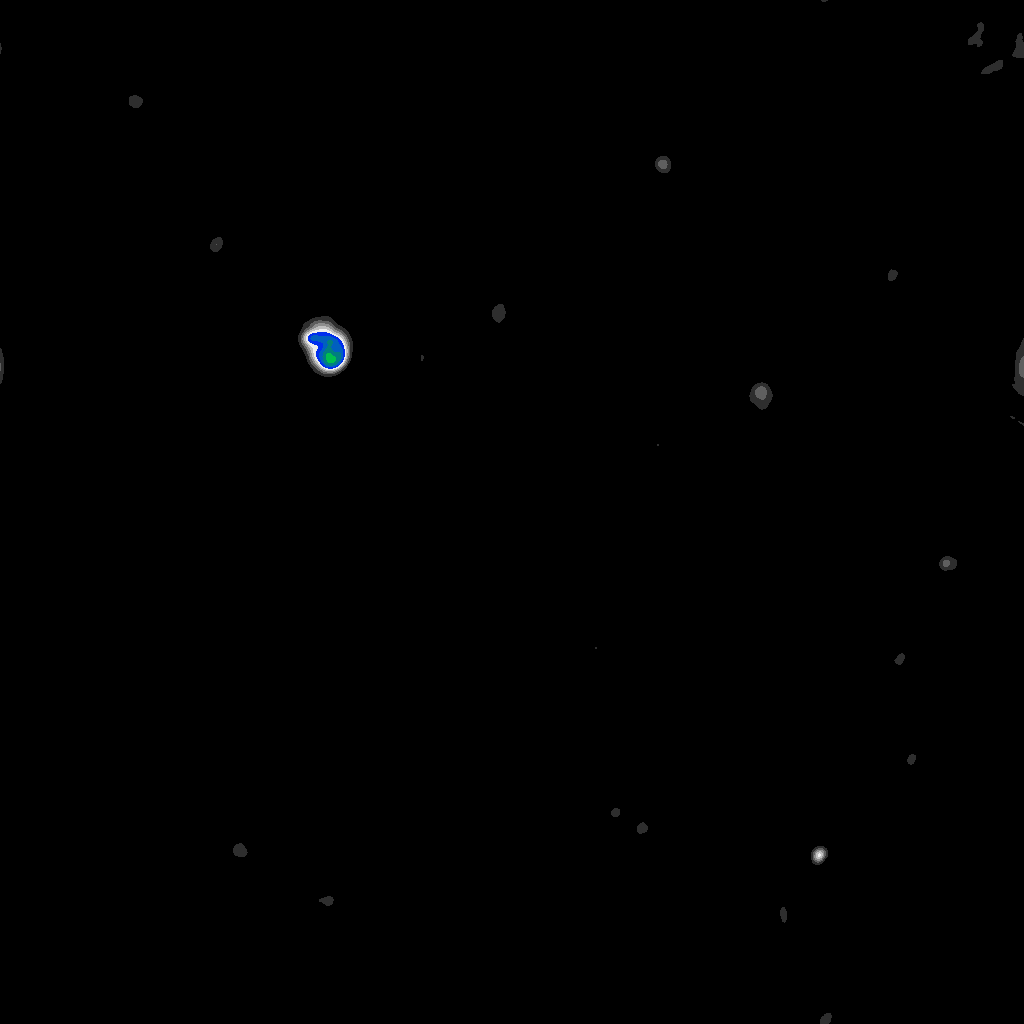
\includegraphics[height=3cm]{./chapters/01.intro/mk2/clean.png}%
		}%
	}
	\setlength{\twosubht}{\ht\twosubbox}
	
	% typeset
	\centering
	\subcaptionbox{Real-world visibilities combined from different channesl and timesteps.\label{intro:inversefig:uvspace}}{%
		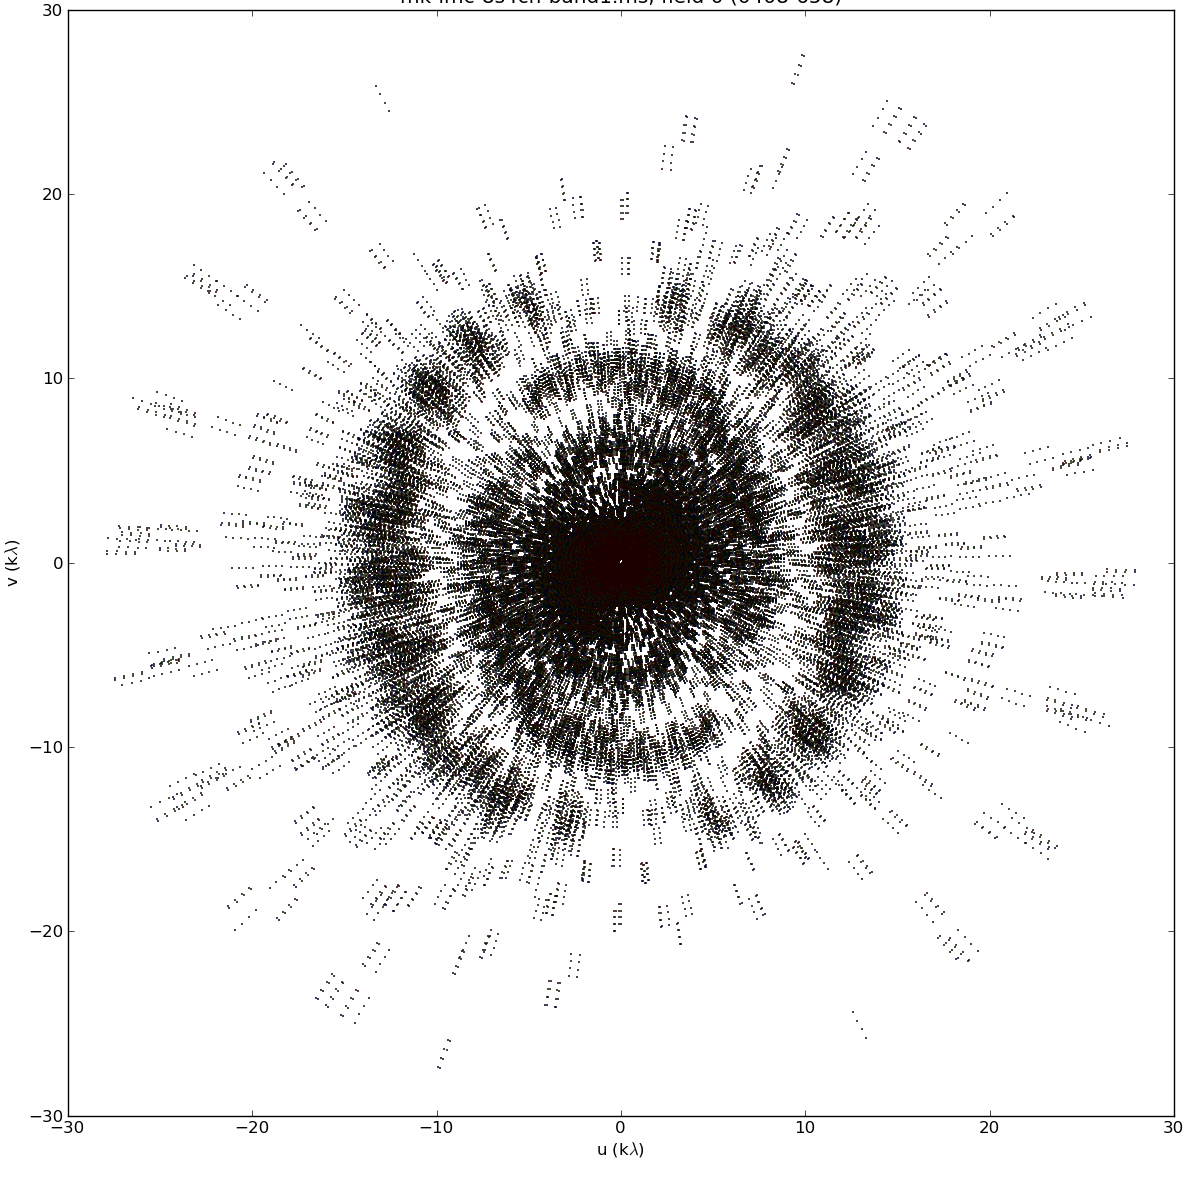
\includegraphics[height=\twosubht]{./chapters/01.intro/meerkat_uv2.png}%
	}\quad
	\subcaptionbox{Reconstruction of the visibility measurements.\label{intro:inversefig:reconstruction}}{%
		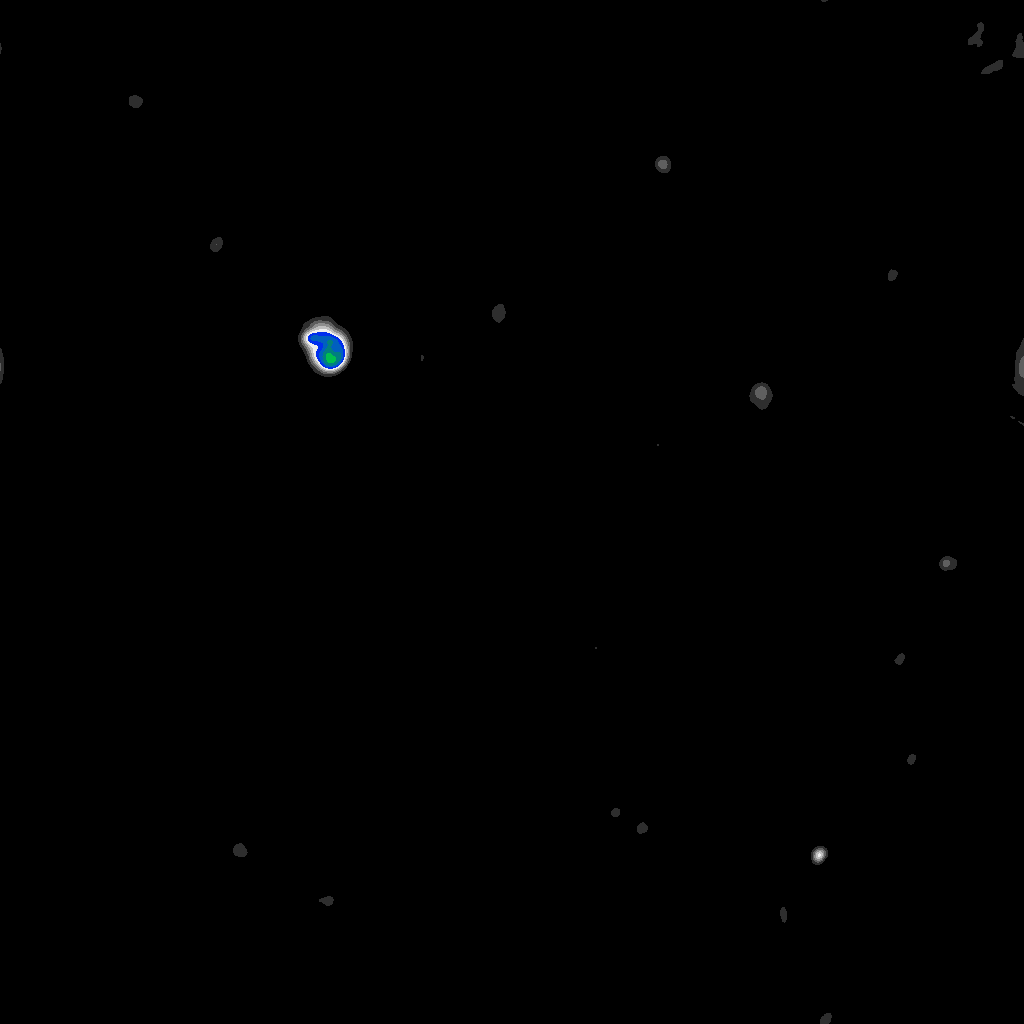
\includegraphics[height=\twosubht]{./chapters/01.intro/mk2/clean.png}%
	}
	\caption{Example of an image reconstruction for Fourier measurements of the MeerKAT radio interferometer}\label{intro:inversefig}
\end{figure}

It is easy to see that the visibility measurements from MeerKAT quickly fills up the hard disk and the Fourier space with samples. The Figure \ref{intro:inversefig:uvspace} shows a fraction of the visibility samples from a real-world observation. The visibilities are combined from multiple channels and multiple timesteps. Although we have a large number of visibilities, we still have areas of the Fourier space without a sample. Although we have a large number of samples, the visibilities are still an incomplete. From the measurements alone, we cannot reconstruct the image shown in Figure \ref{intro:inversefig:uvspace}.

This is known as an ill-posed inverse problem in the literature. A problem is considered ill-posed when:
\begin{enumerate}
	\item No solution exists.
	\item There are solutions, but no unique solution exists.
	\item The solution behavior does not change continuously with the initial condition (For example: a small change in the measurements lead to a very different reconstructed image).
\end{enumerate}
Image reconstruction for radio interferometer is an inverse problem, because we want to find the image which the interferometer observed in Fourier space. It is ill-posed in general, because there are many different images fitting the measurements.

Note that we can reduce the resolution of the reconstructed image until the problem becomes well-posed. The Nyquist-Shannon sampling theorem states the case of radio interferometers: The highest highest Fourier-frequency we measure should be more than twice the highest frequency in the image. The center of the Fourier space in Figure \ref{intro:inversefig:uvspace} is densely sampled. We can reconstruct a low-resolution image that only needs the information from the densely sampled center.

However, this would reduce the effective resolution of the reconstruction. If we can solve the ill-posed inverse problem, we would be able to retrieve the observed image at a higher resolution than possible with the Nyquist-Shannon sampling theorem. As it turns out, this is possible to solve the ill-posed inverse problem by including prior information. We use a numerical optimization algorithm and find the optimal image, which is both consistent with the measurements and consistent with our prior knowledge. This is known in signal processing as compressed sensing \cite{candes2006robust,donoho2006compressed} in the literature. The theory of Compressed Sensing shows that, under the right prior information, we are guaranteed to reconstruct the observed image at a higher resolution than under the Nyquist-Shannon sampling theorem.

%In Section \ref{intro2:ill-posed}, we introduce the Compressed Sensing sampling theorem and show how it works in the case of radio interferometric image reconstruction. The Section \ref{intro2:rec} shows how we can use the theory to create a reconstruction algorithm in practice. But first, we dive deeper into the odds and ends of radio interferometry. 

\subsection{The theory of Compressed Sensing}\label{radio:cs}
We introduce the theory of Compressed Sensing for the problem of radio interferometric image reconstruction. As we have mentioned compressed sensing image reconstruction involves a numerical optimization algorithm to find the optimal solution which is consistent with our measurements and consistent with our prior knowledge. As we will see later, the theory of compressed sensing guarantees us exact reconstruction under certain assumptions. 

Let us formulate the image reconstruction as an optimization problem.The image reconstruction wants to to find the image which is as close to the measurements as possible. Or more formally, we want to minimize the euclidean distance between the visibility measurements $V$ and the reconstructed image $x$. We write it as an objective function:

\begin{equation}\label{radio:cs:l2}
\underset{x}{minimize} \: \left \| V - MFx \right \|_2^2
\end{equation}

Where $F$ is the Fourier transform matrix and $M$ is the "masking" matrix. The Fourier matrix transforms the reconstructed image to visibilities, and the masking matrix zeros out all visibilities that the radio interferometer cannot measure.

We can reconstruct the image by finding the optimum of the objective function \eqref{radio:cs:l2}. The objective function is convex, meaning it has only one global minimum, and we can use the class of convex optimization algorithms to search the minimum. However, our measurements $V$ are incomplete, meaning we do not have all the data we need for reconstruction. This means our objective function \eqref{radio:cs:l2} does not "point" to the observed image. It still has a global minimum, but observed image is not guaranteed to be near the global minimum.

A side note: We are guaranteed to find the observed image at the minimum of \eqref{radio:cs:l2} is when the measurements fulfill the Nyquist-Shannon sampling theorem. In that case, we can find the minimum by calculating the inverse Fourier transform: $x = F^{-1}V$. We can still calculate the inverse Fourier transform when we are dealing with incomplete measurements, but it does not result in the observed image.

However, the objective \eqref{radio:cs:l2} only includes information about the measurements. As we have mentioned before, we have prior knowledge about the image. We know it is likely to contain stars. Stars are radio-emissions which are concentrated around a single pixel. In that case, most pixels of the image will be zero, except for the locations where the interferometer has located stars. In other words, we know that the image is sparse. We can add a regularization to the objective function \eqref{radio:cs:l2} and force the reconstructed image to be sparse. This results in the modified objective function:

\begin{equation}\label{radio:cs:lasso}
\underset{x}{minimize} \: \left \| V - MFx \right \|_2^2 + \lambda \left \| x \right \|_1
\end{equation}

Note the two terms in the objective \eqref{radio:cs:lasso}: We have the same term from our measurements, which we call the "data term". But we also have an additional "regularization term", which is the L1 norm\footnote{Sum of absolute values of the pixels} and forces our reconstruction to be sparse. The parameter $\lambda$ represents how much emphasis we put on the regularization. The new objective function is still convex, it still has a global minimum. The regularization term simply shifted the global minimum to a different location when compared to the first objective \eqref{radio:cs:l2}. Now the question is: How likely is our modified objective \eqref{radio:cs:lasso} to point at the observed image? The theory of Compressed Sensing tells us that it depends on the image content of the observed image. If it only consists of stars, we are practically guaranteed to find the observed image at the minimum of \eqref{radio:cs:lasso}, even though we are dealing with incomplete measurements.

We use the words 'practically guaranteed' because the theory of Compressed Sensing does give us guarantees to find the observed image at the minimum of \eqref{radio:cs:lasso} under certain assumptions. The issue is these assumptions are hard to verify for any given reconstruction problem. In reality, it is often easier to empirically show that the regularization works. For example, by creating a super-resolved\footnote{The radio interferometer also has a resolution limit. Super-resolved reconstructions were able to find structures which are smaller than the limit of the instrument.} reconstruction from visibility measurements \cite{dabbech2018cygnus}. The assumptions do have important implications for instrument design. This project however is focused on the numerical optimization algorithm. We do not have an influence on the visibility measurements, for our intends and purposes, the measurements are fixed. That is why we first give an intuitive explanation to when the observed image is at the minimum of the objective \eqref{radio:cs:lasso}, and what this means for the ill-posed image reconstruction next. Then we give an overview of the formal guarantees in Section \ref{radio:cd:formal} and the implications for the visibility measurements.


\subsubsection{Exact reconstruction in theory}\label{radio:cd:intuitive}
What is exact reconstruction: When the most likely image is equal to the observed image. 

Let us go back to our example of an image containing only stars. Let us say it has $256^2$ pixels and contains $S = 10$ stars. But we do not know how many it has, where they are, nor their intensity (pixel value). We just know there ara only stars in the image. 

If we measure the image with a single-dish instrument, we measure every pixel after each other. Note that, because we know the image contains only stars, we already know most pixels will be zero. When the single-dish measures a zero pixel, all we learn is that there is no star at this location. We only learn something vital when the single-dish instrument hits one of the 10 stars. We learn little when the instrument measures a zero pixel, and a lot when it measures a pixel with a star. On average over all pixel measurements, we learn little about the image.

%Image of fourier measurements

When we measure the image with a radio interferometer, we measure visibilities (Fourier components) of the image. Remember that a single visibility is a measurement over the whole image. Every pixel of the image has contributed to the amplitude and phase of the visibility. Every visibility measurement contains some information about the 10 stars in the image. On average, each visibility measurement contains more information about the stars than the average pixel measurement of the single-dish instrument.

T

Randomly sampling the visibilities tends to be optimal.

The question that remains is: What visibilities, and how many do we need to reconstruct our image? The answer depends on two components: It depends if the matrix $F$ of our objective \eqref{radio:cs:lasso} fulfills the Restricted Isometry Property (RIP) and on the number of stars in the image.

The Restricted Isometry Property (RIP)\cite{candes2006robust,donoho2006compressed} basically says that a random subset of columns in $F$ have to be (approximately) uncorrelated. 
In our example with an image containing 10 stars, it means that each star is uncorrelated from each other.
Another example: they have to be roughly orthogonal.
If we have found a solution with 10 stars, the RIP is the tool to prove that there exists no solution with fewer stars. Therefore the solution is optimal.

At what point we fulfill the RIP also depends on the number of stars. Intuitively this makes sense. We do not need as many data if the image is simple.
Note on sparseness: also possible in different spaces. Funny thing, when we find a space which the image is even more sparse, we need even less visibility measurements for reconstruction.

If we randomly sample the Fourier space, the resulting matrix $F$ is likely to fulfill the RIP\cite{haviv2017restricted}. Likely means for all practical purposes, it might as well be guaranteed.


\subsubsection{Exact reconstruction in practice}
Interferometer does not sample randomly, and does not only contain stars.

A radio interferometer does not randomly sample the visibilities. As we have seen, the sampling pattern depends on the antenna layout of the interferometer. For us, the matrix $F$ of a reconstruction problem is fixed, and cannot be changed after the observation is recorded.
Do not have the guarantees. But that is not too bad, we may not need the RIP. 
 Exact reconstruction can also work under less strict conditions\cite{candes2011probabilistic}.
 
What to do about extended emissions. It is a data modelling task, how do we find good regularization that leads to the sparset result possible. Problem of validation, we do not know the best regularization beforehand. We can only choose one that works "well.

The theory of compressed sensing gives us a framework. There is a data modelling task, and a task for finding efficient algorithms.

So there is a data modelling task in finding a good sparse prior.
We also do not know the proper sparse space in which radio interferometric images. We know several spaces, Curvelets \cite{starck2003astronomical} Starlets \cite{starck2015starlet}, Daubechies wavelets \cite{carrillo2012sparsity}. As of the time of writing, it is currently unknown which leads to the best reconstruction.
We can also learn dictionaries.


%\subsubsection{General Compressed Sensing reconstruction formulation}
%Use everything with the L1 norm. More general formulation
%$F$ is fixed, because we cannot change the interferometer.
%We do just need a sparse space.


\subsection{Noise, approximations and other difficulties in radio interferometry}
We give a short introduction into how the electromagnetic wave gets measured by the interferometer, turned into visibilities and finally processed into an image. Figure \ref{intro:system} shows a radio source and its electro-magnetic (em) wave arriving at the antennas of the interferometer. It then shows the three processes involved to arrive at an image: Correlation, calibration and image reconstruction.
	
\begin{figure}[h]
	\centering
	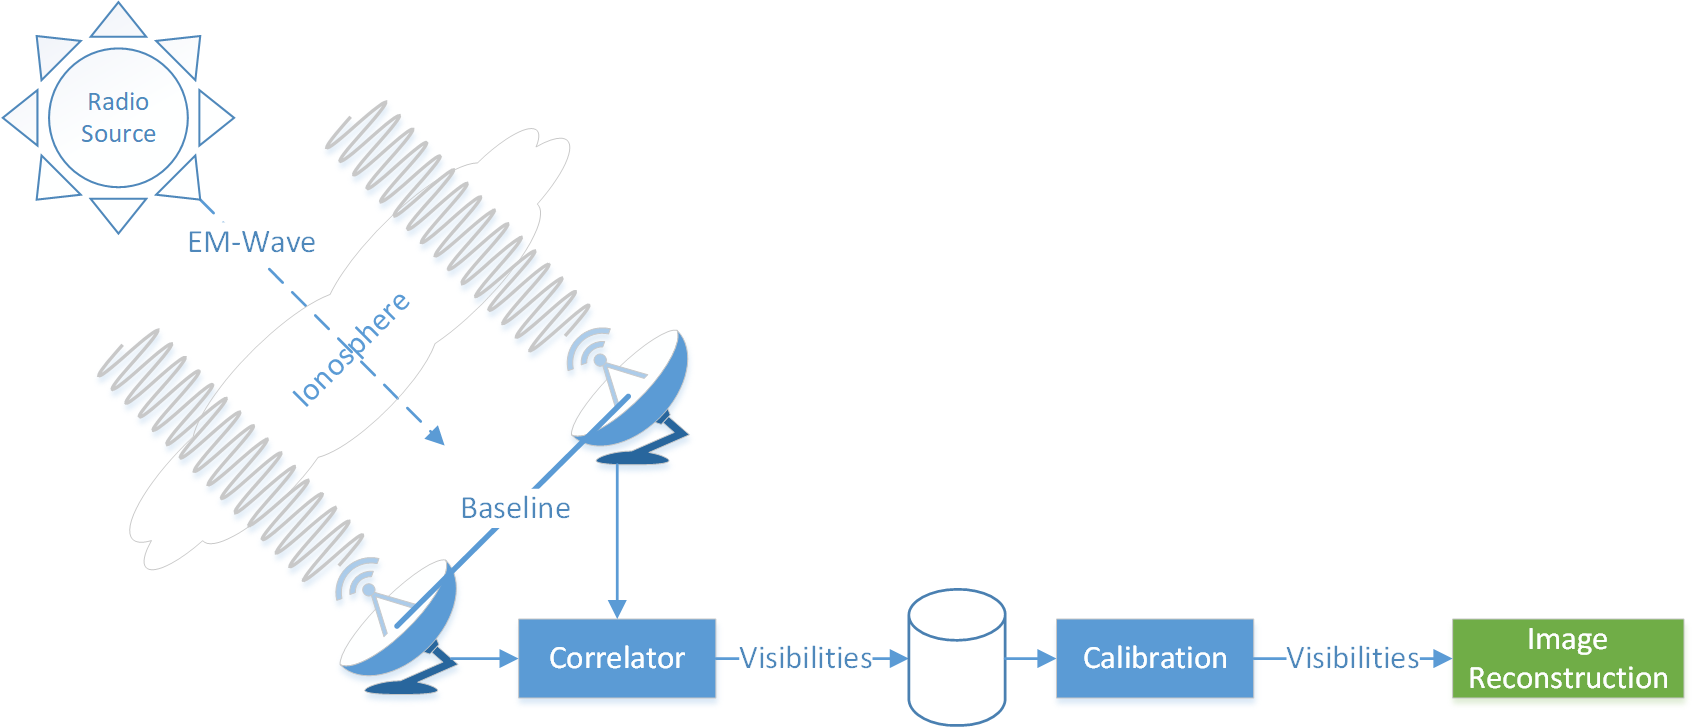
\includegraphics[width=0.80\linewidth]{./chapters/01.intro/system.png}
	\caption{Radio interferometer system}
	\label{intro:system}
\end{figure}

First, we have a source in the sky that is emitting em-waves in the radio frequency. The waves travel to earth, through the earth's ionosphere and finally to our interferometer. Along its path, the e-m waves may get distorted from various sources. For example, it may receive a phase shift by the ionosphere.

Then, the em-wave arrives at our interferometer. We call each antenna pair a baseline. Each baseline will end up measuring a single visibility. The distance between the antennas and their orientation to the em-wave will determine where we sample the $uv$-plane. Short baselines measure the $uv$-plane close at the origin, while long baselines sample the $uv$-space further away from the origin. Remember that the samples away from the $uv$-origin contain the information about edges and other details of our image. With a longer baseline the interferometer measures more highly resolved details, regardless of the antenna dish-diameter\footnote{Remember that this is the reason why we build radio interferometers. We do not need impossibly large dish diameters for a high angular resolution. We just need large distances between smaller antennas.}. The figure \ref{intro:system} shows the em-wave arriving at a single baseline of the interferometer. Each antenna picks up its version of the em-wave and transfers it to the correlator.

The correlator then takes the feed of each antenna and correlates the signals, which results in the amplitude and phase of the visibility component. Amplitude and phase for each visibility are measured for a short time range (i.e. fractions of a second up to several seconds). At this point, the visibilities are saved to disk for further processing. The radio interferometer produces a visibility measurement for each baseline, for each time range, for each frequency channel of the instrument. Because a single observation can take up to several hours, measured with several thousand frequency channels, radio interferometers produce an almost arbitrary large number of visibilities.

Calibration

Image Reconstruction

%Calibration. Effects from the ionosphere. Imperfections of the instrument, like varying antenna sensitivity.
%Calibration is complex, and not part of the project

%Image reconstruction generally happens after calibration. The focus of this project.
%self-calibration

\subsubsection{The measurement equation}
As we discussed so far, the radio interferometer measures visibilities of the sky image, and we wish to find the observed image from the measurements. Put formally, we wish to invert the following system of linear equations \eqref{intro2:model:linear}, where $V$ is the visibility vector\footnote{We use the lower-case $v$ to denote the axis in the Fourier space $uvw$, and the upper-case letter to denote the visibility vector.}, $F$ is the Fourier transform matrix and $I$ is the pixel vector of the observed image.

\begin{equation}\label{intro2:model:linear}
V = F I
\end{equation}

We wish to find the observed image $I$, while we only know the visibility vector $V$ and the Fourier transform matrix $F$. This is what we call the measurement equation. In most context for this project, looking is an adequate view of the image reconstruction problem. We will show why we cannot find the observed image $I$ by simply calculating the inverse Fourier transform. However, when we need to efficiently apply the Fourier transform, we need to know $F$ in more detail. As we will see, radio interferometers have some difficulties hidden in the Fourier transform matrix, which are difficult to handle efficiently. First, let us abandon the vector notation of \eqref{intro2:model:linear}, and represent the measurement equation with integrals \eqref{intro2:model:smallfov}.

\begin{equation}\label{intro2:model:smallfov}
V(u, v) = \int\int I(l, m)  e^{2 \pi i [ul+vm]} \: dl \: dm
\end{equation}

This is essentially the same problem. The main difference is that we do not represent the Fourier transform as a matrix $F$, but as integrals $\int\int e^{2 \pi i [ul+vm]}$, where $u$, $v$ are the coordinates in Fourier space and $l$, $m$ are the angles away from the image center. A single pixel represents the intensity of the radio emission from the direction $l$, $m$. Note that the measurement equation \eqref{intro2:model:smallfov} shows the fact that the visibilities are measured in a continuous Fourier space. If the Fourier space would also be discrete, we could replace the integrals with sums.

However, the measurement equation \eqref{intro2:model:smallfov} is inaccurate in the sense that it ignores many effects that distort the signal. For example, it does not account for the distortion by the ionosphere, or the distortion introduced by real-world antennas. The measurement equation \eqref{intro2:model:smallfov} shown here does not represent the real world. But depending on the instrument and the observation, these distortions may be negligible, and the measurement equation \eqref{intro2:model:smallfov} is a good approximation. 

When there is a distortion source that cannot be ignored, it has to be modelled in the measurement equation. As such there is no unified measurement equation for all radio interferometric observations, let alone radio interferometers. The equation shown in \eqref{intro2:model:smallfov} can be seen as the basis that gets extended as necessary\cite{smirnov2011revisiting1, smirnov2011revisiting2, smirnov2011revisiting3, smirnov2011revisiting4}.

For example, the measurement equation \eqref{intro2:model:smallfov} is only accurate for small field of view observations, when $l$ and $m$ are both small angles. For wide field of view observations, we need to account for the fact that the visibilities have a third term $w$, and we arrive at the wide field of view measurement equation \eqref{intro2:model:widefov}.
 
\begin{equation}\label{intro2:model:widefov}
 V(u, v, w) = \int\int  \frac{I(l, m)}{c(l, m)}  e^{2 \pi i [ul+vm+ w(c(x, y) - 1)]} \: dl \: dm \:,  \quad c(l,m) = \sqrt{1 - l^2 - m ^2}
\end{equation}
 
The third $w$-term has two effects on the measurement equation. It introduces a phase shift in the Fourier transform $e^{2 \pi i [\ldots +w(c(l, m) - 1)]}$, and a normalization factor of the image $\frac{I(l, m)}{c(l, m)}$. Note that when the angles are small, i.e. $l^2 +m^2 \ll 1$ then the wide field of view measurement equation \eqref{intro2:model:widefov} reduces to our original \eqref{intro2:model:smallfov}. This is another way of saying that for small field of views, the measurement equation \eqref{intro2:model:smallfov} is a good approximation under the right conditions. 

In this project, we use the wide field of view measurement equation \eqref{intro2:model:widefov}. But as we mentioned in the beginning of this section, for most contexts, it is not important whether we ignore the $w$-term of the visibilities or not. It is important when we design an efficient implementations for applying the wide field of view Fourier transform, because the $w$-term keeps us from using the Fast Fourier Transform (FFT). In every other case, we can ignore this technicality. Because even more complicated measurement equation still have a linear relationship between visibilities and image \cite{smirnov2011revisiting1, smirnov2011revisiting2, smirnov2011revisiting3, smirnov2011revisiting4}. We can view the whole reconstruction problem as a system of linear equations \eqref{intro2:model:linear}, where the matrix $F$ takes care of how exactly the measurements and pixels relate in this case.



\subsubsection{Image reconstruction algorithm}\label{intro2:rec}
This section explains the most wide spread reconstruction algorithm and their general architecture. 

The objective function \eqref{radio:cs:lasso} of the previous section both contains the visibility measurements $V$ and the image $x$. The Fourier transform matrix $F$ represents the relationship between the visibilities $V$ and image $x$. 

\begin{equation}
\begin{split}
\underset{x}{minimize} &\: \left \| V - MFx \right \|_2^2 + \lambda \left \| x \right \|_1 \\
\underset{V_2}{minimize} &\: \left \| V - MV_2 \right \|_2^2 + \lambda \left \| F^{-1}V_2 \right \|_1
\underset{x}{minimize} &\: \left \| I_{dirty} - x * PSF \right \|_2^2 + \lambda \left \| x \right \|_1
\end{split}
\end{equation}



Remember that most reconstruction problem in radio astronomy have far more visibility measurements than pixels in the reconstruction. This can be exploited by the reconstruction algorithm. 

\subsubsection{CLEAN deconvolution algorithm}

CLEAN deconvolutions algorihm

Problem

\subsubsection{The Major/Minor cycle}\label{intro2:opt:cycle}


